\chapter{Evidence trajectory: 무엇이 실제로 성숙하고 있는가}
\label{STC-S09}

이 장의 목적은 논문 수를 세어 momentum을 선언하는 것이 아니라, 서로 다른 종류의 증거가 어떤
주장을 허용하는지 분리하는 것이다. 연구용 알고리즘의 controlled experiment, 공개 code, 공식
product documentation, production trace, independent incident report는 같은 무게가 아니다. 또한
``sleep''이라는 단어가 없는 continual learning, external memory, state caching 연구도 lifecycle의
일부를 직접 다룰 수 있고, 반대로 생물학적 은유만 사용하는 연구는 operational STC의 증거가 아닐 수
있다.

\section{Date-frozen corpus와 재현 가능한 경계}

본 연구는 2026-08-05를 source freeze로 고정했다. Registry에는 paper, official release,
documentation, tagged repository를 합쳐 73개의 primary/official source가 들어 있다.
\claim{STC-C001} 각 source는 stable ID, canonical URL, 공개일, 접근일, source type을 가지며, 본문의
claim은 prose citation이 아니라 마지막 ledger의 exact locator로 다시 연결된다. 이 수는 검색 결과의
개수가 아니라 중복 제거와 source-kind 판정을 마친 audit surface다.

동결 시점에 명시적 background memory synthesis를 설명한 공개 production lineage는 적어도
OpenAI Dreaming과 Mem0 Dream 두 개였다.\claim{STC-C002}
\autocite{srcstc0052,srcstc0063} Letta의 tagged sleeptime code와 Zep/Graphiti의 temporal provenance는
같은 lifecycle을 다른 component에서 보강하지만, product-scale comparative effectiveness를 대신하지
않는다. 공식 release는 ``기능이 존재한다''를 지지할 수 있어도 ``strongest baseline보다 우월하다''를
지지하지 못한다.

검색은 saturation을 과장하지 않는다. 12개 cluster 중 2개만 bounded closure, 5개는 active frontier,
5개는 measurement gap으로 닫혔다.\claim{STC-C003} 특히 utility--sleep compute, utility--memory
budget, retention--update count, bytes moved--placement curve가 없는 cluster는 source가 많아도
``saturated''로 부르지 않았다. 이 규칙은 2026-08-05 이후의 발견이 결론을 바꿀 수 있음을 문서 구조에
남긴다.

\section{Evidence maturity와 expected value는 다른 축이다}

\begin{table}[htbp]
\centering
\caption{본문에서 사용하는 evidence maturity ladder}
\label{tab:evidence-ladder}
\begin{tabularx}{\textwidth}{C{0.09\textwidth} L{0.28\textwidth} Y Y}
\toprule
Level & 최소 근거 & 허용되는 문장 & 허용되지 않는 확대 해석 \\
\midrule
E0 & 아이디어·명칭 & 제안되었다 & 작동한다 \\
E1 & 단일 synthetic/offline 실험 & 제한된 setting에서 관측됐다 & 일반화된다 \\
E2 & 다중 task/model 또는 code & 조건부로 지지된다 & production-ready다 \\
E3 & strong baseline, ablation, long horizon & 평가 범위에서 경쟁력 있다 & fleet economics가 성립한다 \\
E4 & 공식 production lifecycle & 공개 제품에서 동작한다 & scientific optimum이다 \\
E5 & independent deployment trace·incident & 운영 성질이 독립 확인됐다 & 다른 workload에도 보편적이다 \\
\bottomrule
\end{tabularx}
\end{table}

Expected value가 높아도 evidence가 E1이면 high-upside research bet이다. 반대로 E5인 query-time
retrieval이 특정 high-reuse procedural workload에서 가장 값싼 해답이라는 뜻도 아니다. 본 논문은
problem severity, quality advantage, cost advantage, evidence maturity, deployment fit, governance,
industry momentum, academic momentum을 각각 기록하고 평균 점수 하나로 숨기지 않는다.

\section{Industry와 academia의 서로 다른 수렴}

\begin{figure}[htbp]
  \centering
  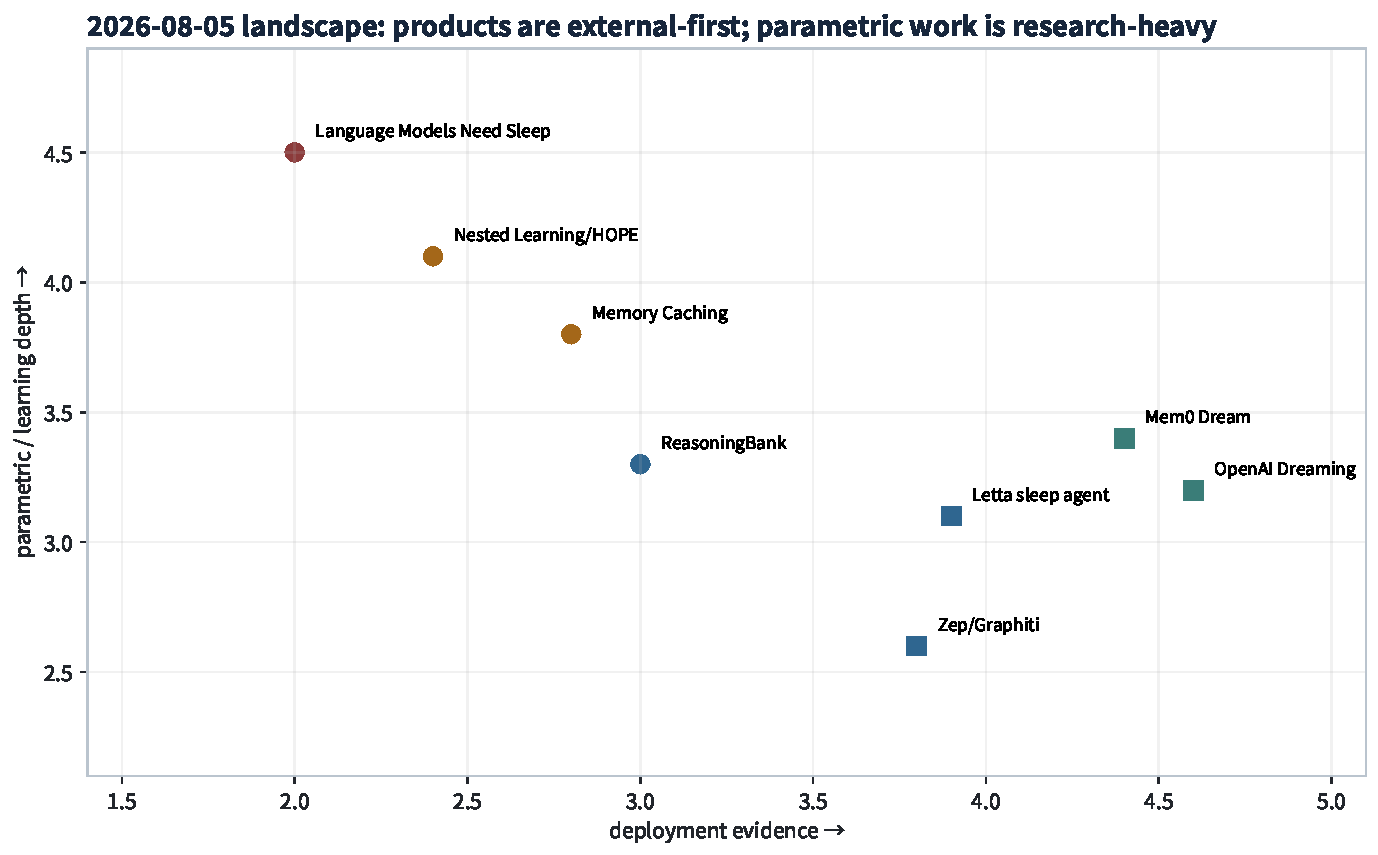
\includegraphics[width=0.96\textwidth]{figures/stc-f014.pdf}
  \caption{Source freeze 시점의 industry--academia landscape. Industry는 external synthesis와
  temporal provenance에, academia는 continual learning, neural memory, learned writer와 capacity
  theory에 더 넓게 분포한다. 좌표는 corpus의 정성적 audit를 시각화한 것이며 시장 규모가 아니다.}
  \stcfigure{STC-F014}
  \figsource{Original synthesis; SRC-STC-0054, SRC-STC-0056, SRC-STC-0057}{제품과 연구 lineages를 external lifecycle, learned memory policy, parametric consolidation, benchmark/theory 축에 배치한 지도.}
  \label{fig:industry-academia}
\end{figure}

Industry에서 가장 분명한 경로는 episode 보존 $\rightarrow$ contradiction/dedup $\rightarrow$
scheduled pattern synthesis $\rightarrow$ future retrieval $\rightarrow$ user control/provenance다.
Academia의 경로는 더 넓다. Replay와 continual-learning regularization, test-time neural memory,
memory writer/router RL, rate--distortion compaction, self-evolving strategy memory, sequential fact
reachability가 서로 다른 이름으로 같은 admission--transform--destination--validation 문제를 만든다.
\autocite{srcstc0020,srcstc0021,srcstc0035,srcstc0043,srcstc0051}

따라서 momentum에 대한 정확한 표현은 ``external background transformation은 I3/E4에 도달했고,
learned external policy는 빠른 E2--E3 frontier이며, broad per-user parametric sleep은 E1--E2''다.
이 세 문장을 하나의 ``STC가 뜬다''로 합치면 투자 방향과 실험 설계가 모두 왜곡된다.

\section{번역 corpus가 담당하는 역할}

전체 source를 모두 번역하는 대신, explicit sleep, biological/computational precursor, continual
learning, external memory, neural memory, capacity, negative evidence를 가로지르는 15편을 balanced
translation corpus로 고정했다.\claim{STC-C004} 번역본은 의견을 추가하는 secondary review가 아니라
원문의 section·figure·limitation을 보존하는 독해 보조물이다. 반면 이 Study는 그 source들을
problem과 lifecycle 기준으로 재조합하는 분석이다. 두 산출물을 분리해야 번역자의 해석이 원저자의
주장처럼 보이지 않는다.

\begin{keypoint}[Evidence trajectory의 결론]
새로운 축의 가장 강한 증거는 하나의 breakthrough paper가 아니다. Continual-learning mechanism,
external-memory product, asynchronous implementation, temporal provenance, realistic benchmark가 서로
다른 층에서 같은 lifecycle boundary를 채우기 시작했다는 점이다. 다만 parametric destination의
장기 retention·delete·rollback·fleet cost를 동시에 보여 주는 공개 증거는 아직 비어 있다.
\end{keypoint}
